\begin{figure*}[htbp]
    \centering
    \begin{subfigure}[t]{0.32\textwidth}
        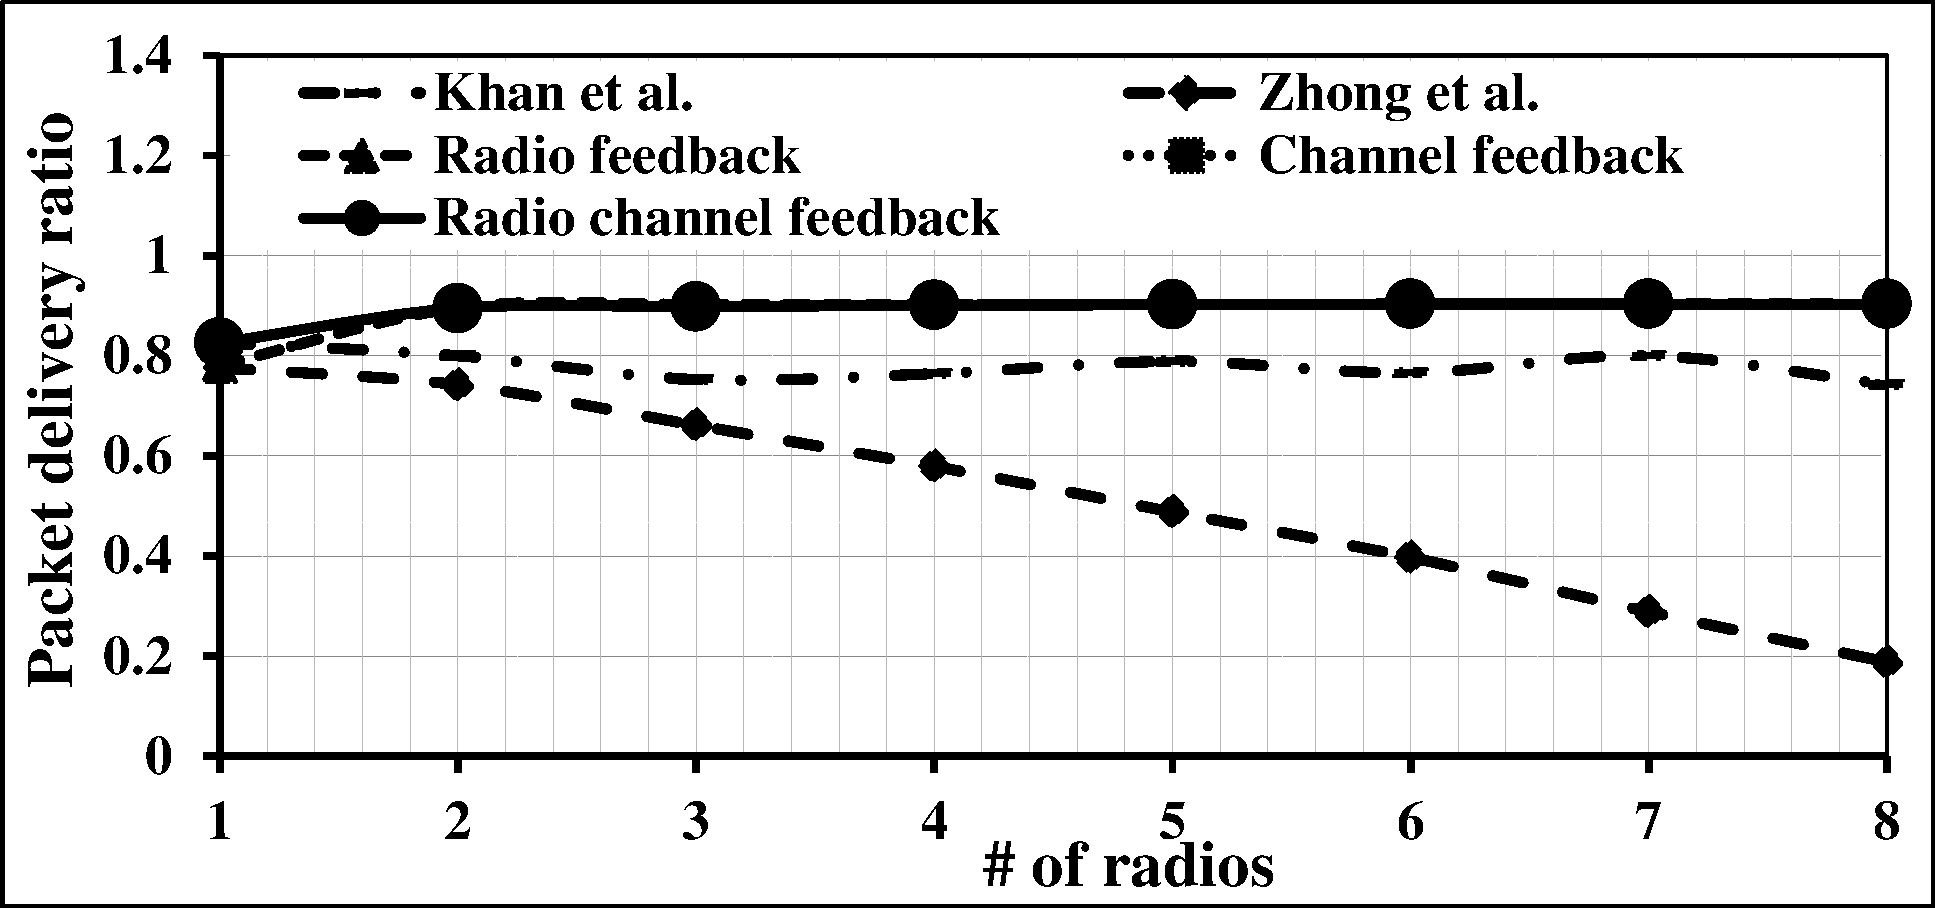
\includegraphics[width=\textwidth]{topology4/DeliveryRatio24d1}
        \caption{1Mbps application data rate}
        \label{fig:topology4PD1}
    \end{subfigure}
    ~
    \begin{subfigure}[t]{0.32\textwidth}
        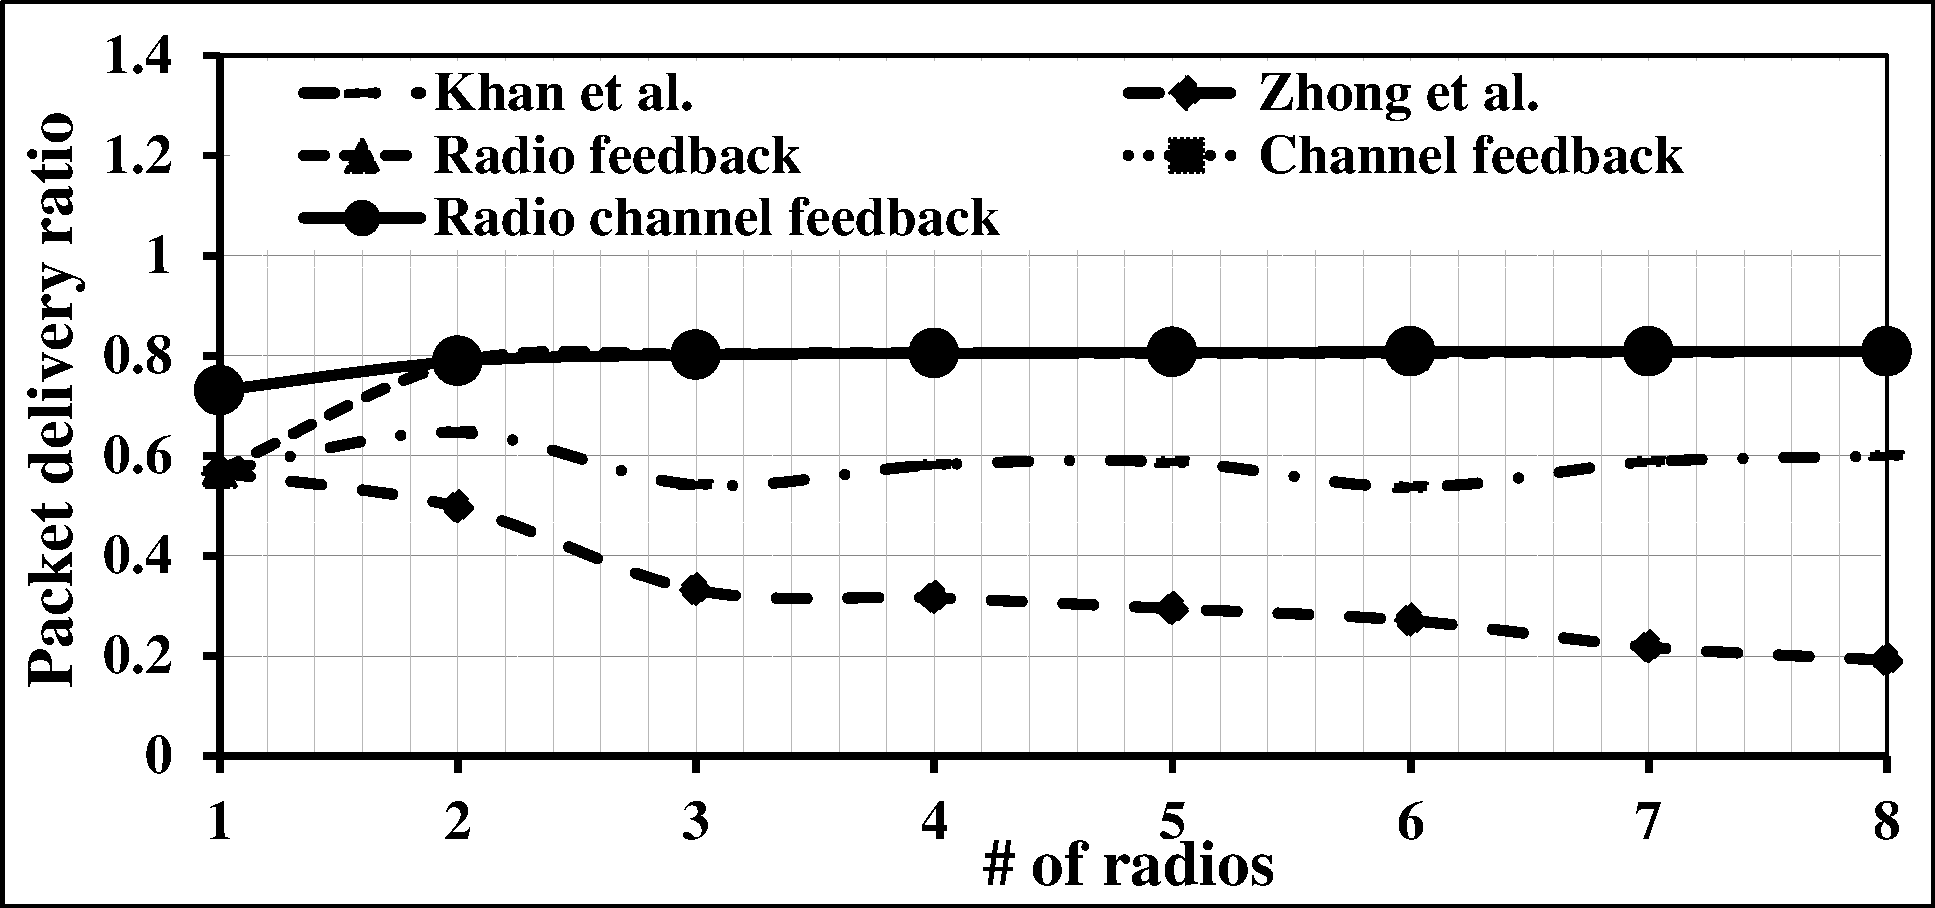
\includegraphics[width=\textwidth]{topology4/DeliveryRatio24d2}
        \caption{2Mbps application data rate}
        \label{fig:topology4PD2}
    \end{subfigure}
    ~
    \begin{subfigure}[t]{0.32\textwidth}
        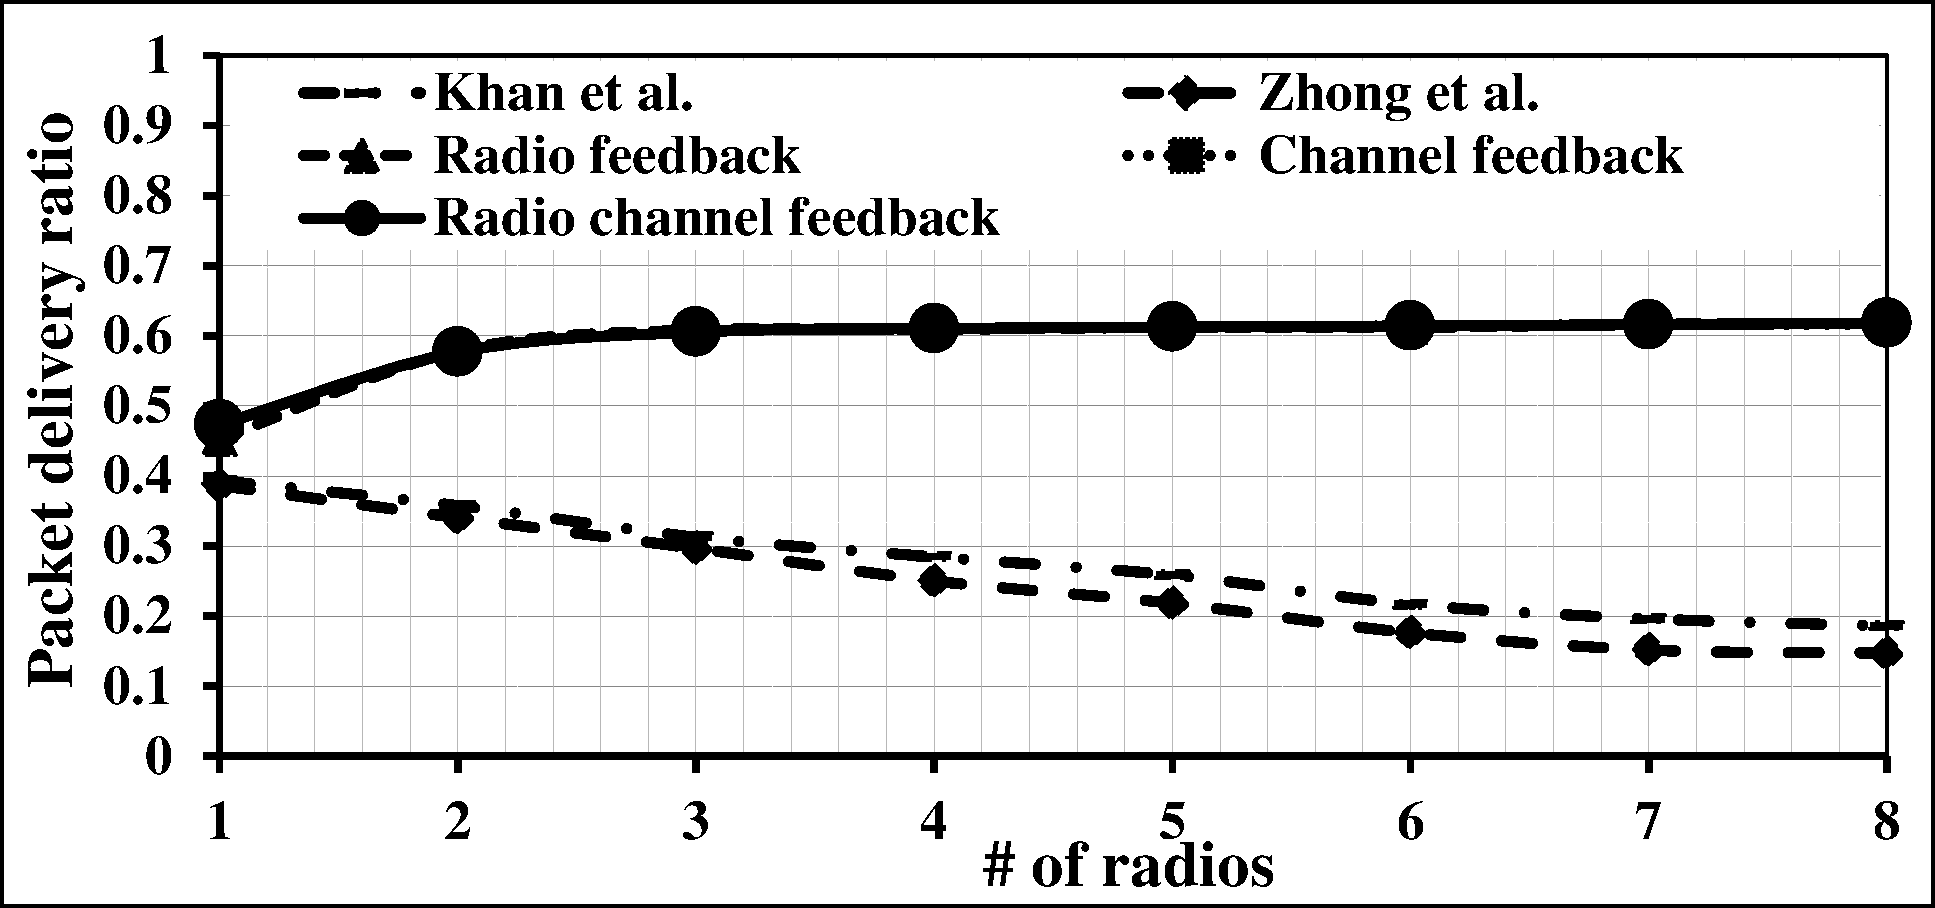
\includegraphics[width=\textwidth]{topology4/DeliveryRatio24d4}
        \caption{4Mbps application data rate}
        \label{fig:topology4PD3}
    \end{subfigure}
    ~\\
    \begin{subfigure}[t]{0.32\textwidth}
        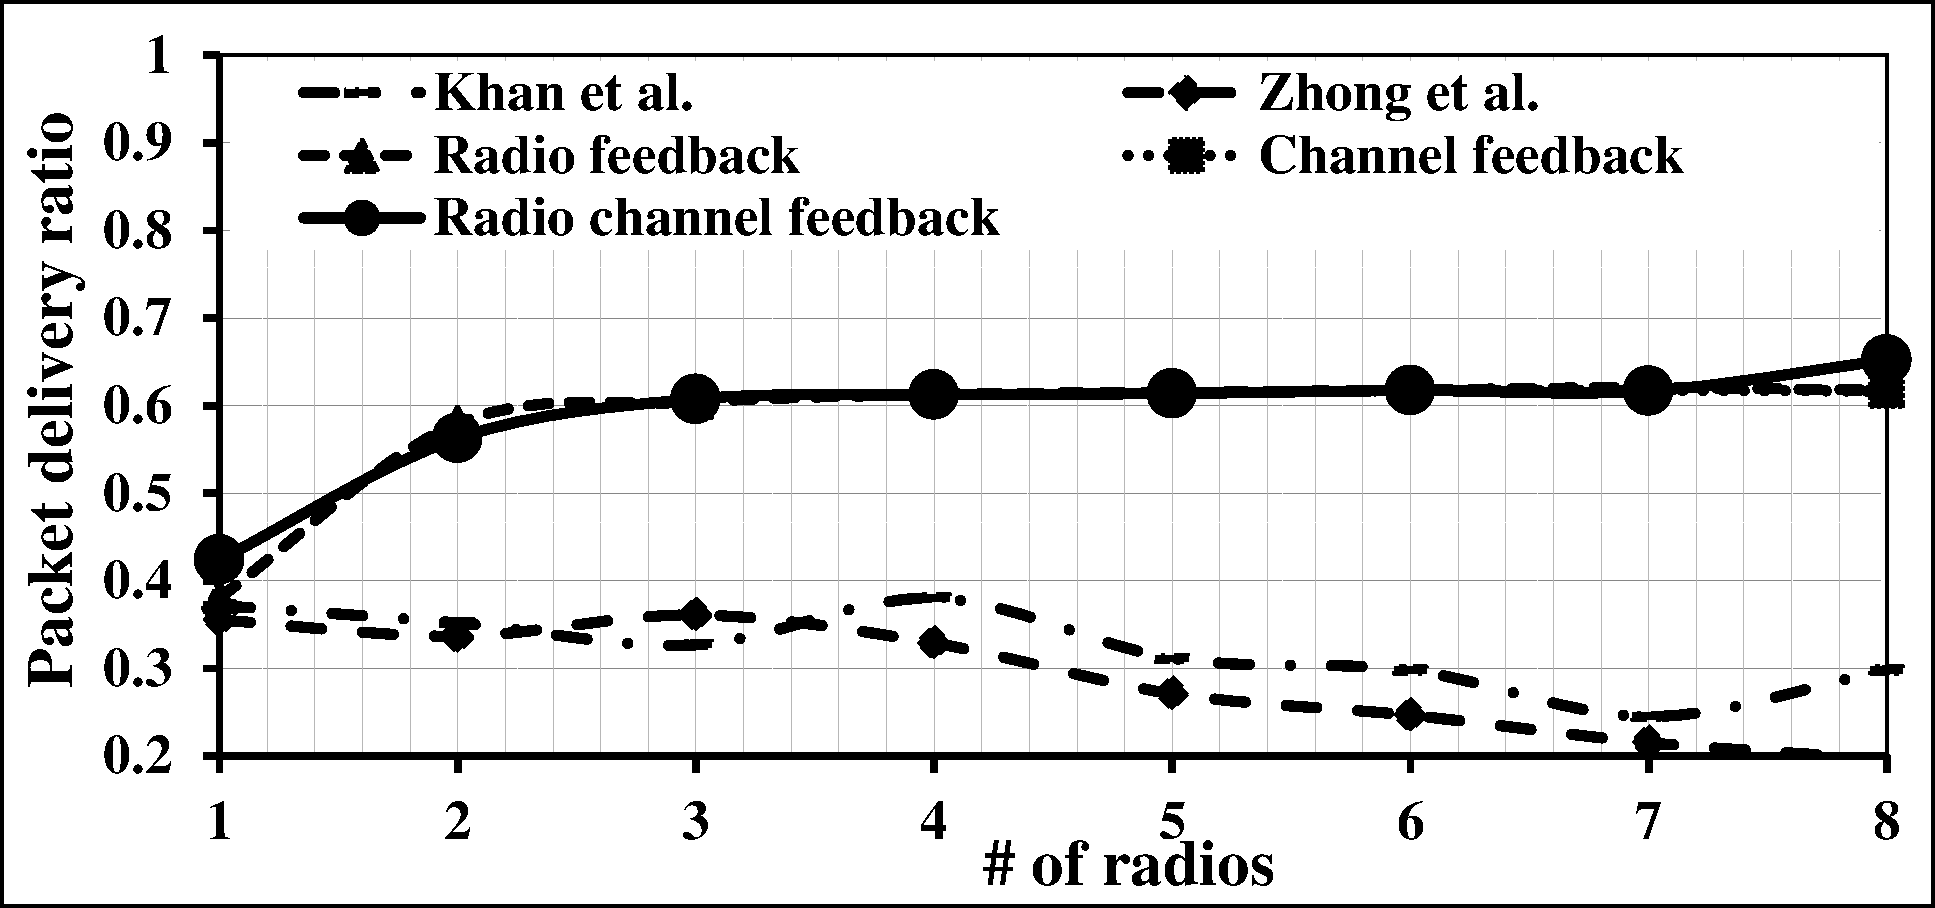
\includegraphics[width=\textwidth]{topology4/DeliveryRatio24d8}
        \caption{8Mbps application data rate}
        \label{fig:topology4PD4}
    \end{subfigure}
    ~
    \begin{subfigure}[t]{0.32\textwidth}
        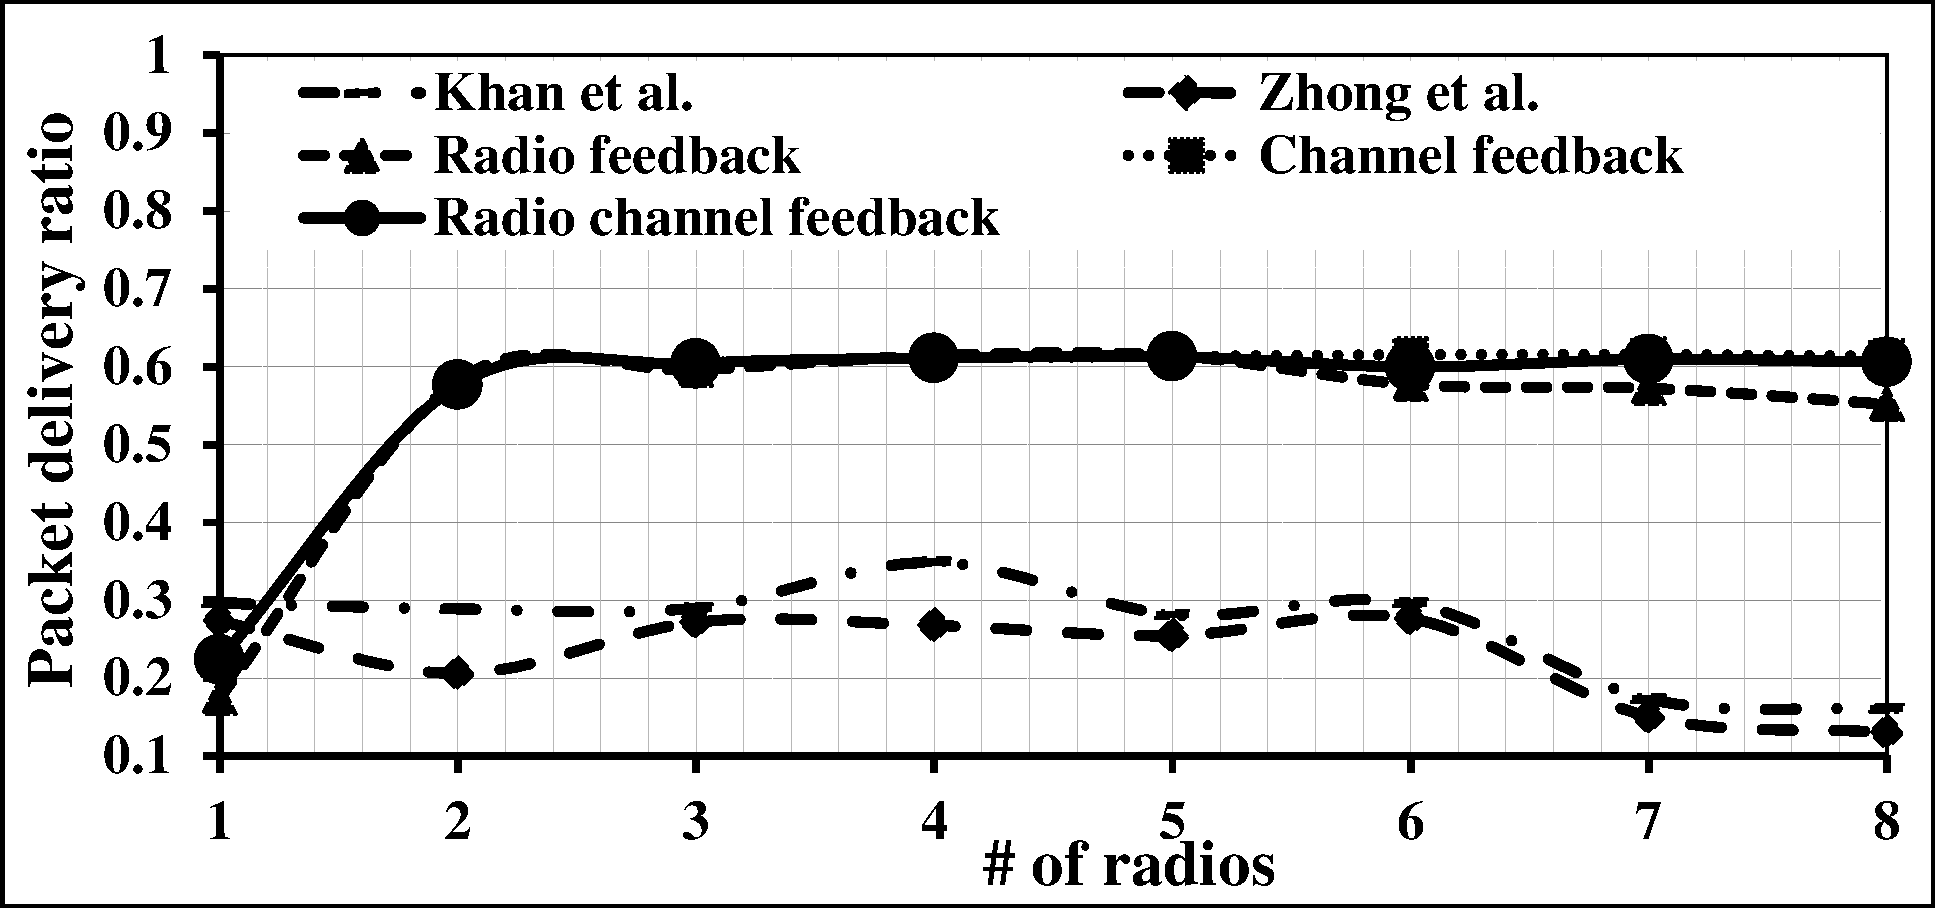
\includegraphics[width=\textwidth]{topology4/DeliveryRatio24d16}
        \caption{16Mbps application data rate}
        \label{fig:topology4PD5}
    \end{subfigure}
    ~
    \begin{subfigure}[t]{0.32\textwidth}
        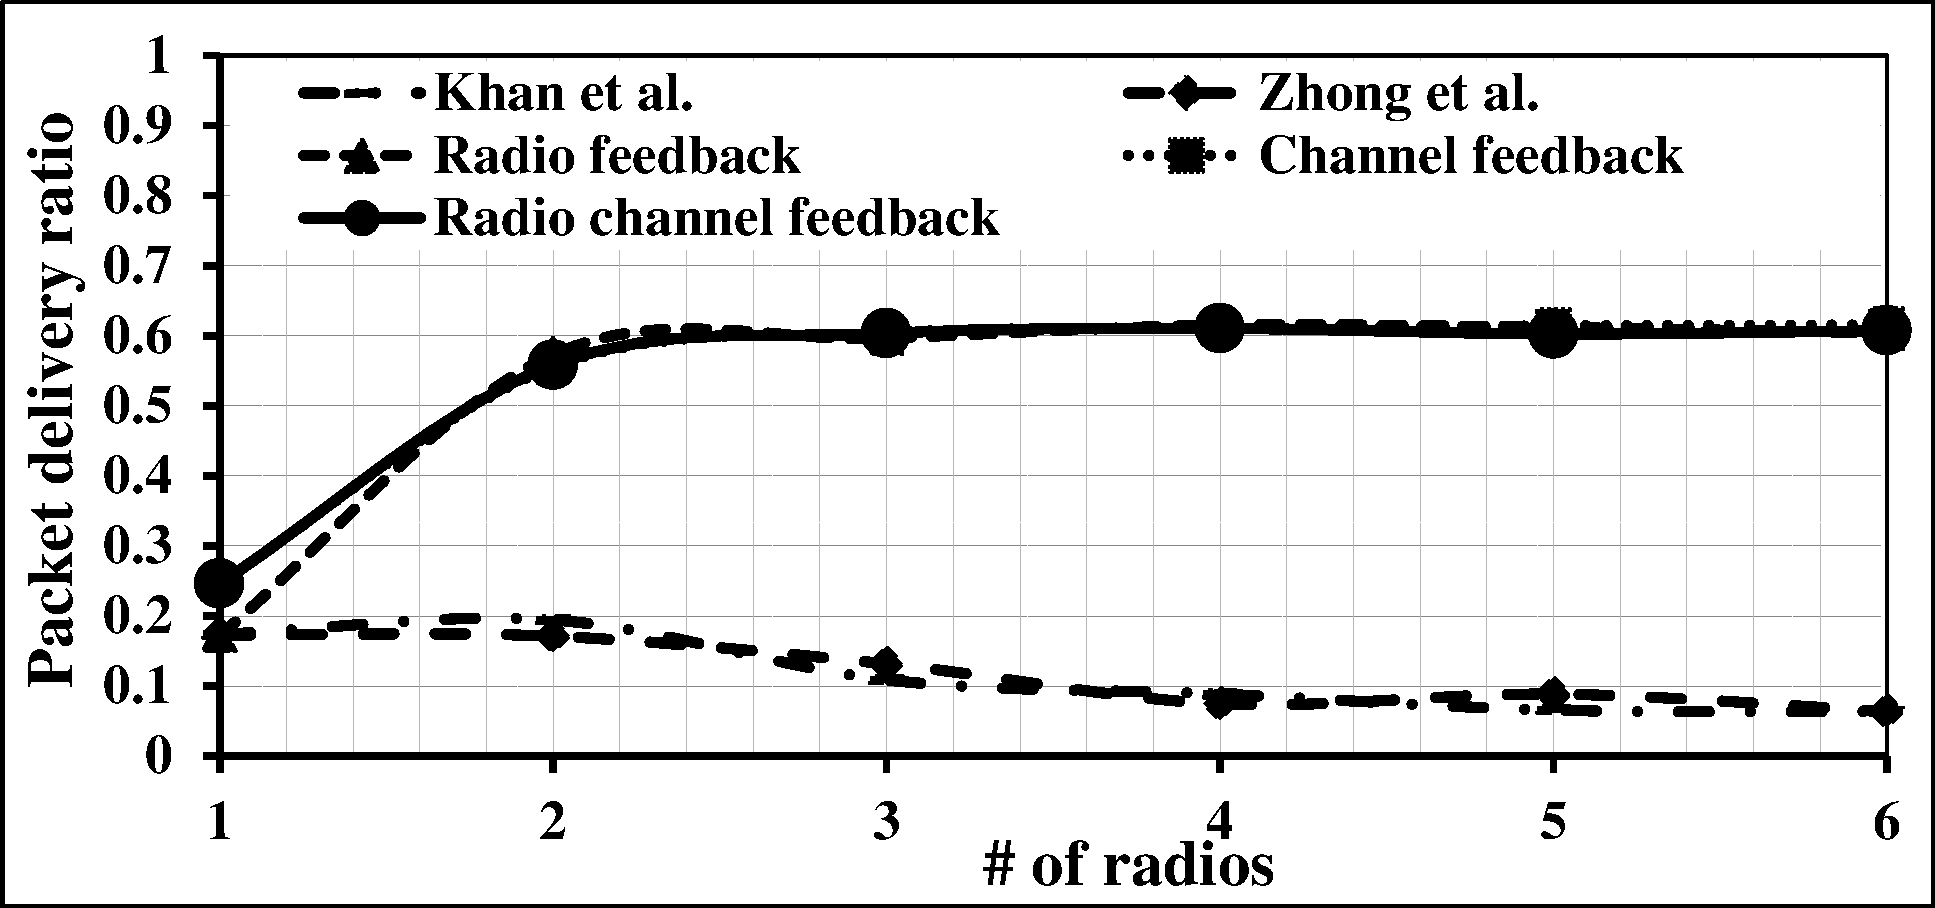
\includegraphics[width=\textwidth]{topology4/DeliveryRatio24d32}
        \caption{32Mbps application data rate}
        \label{fig:topology4PD6}
    \end{subfigure}
    \caption{Application layer packet delivery ratio with varying number of radios for various application data rates}
    \label{fig:topology4PD}
    \vspace{-0.5cm}
\end{figure*}
